\documentclass[a4paper, 12pt]{report}
\usepackage[brazilian]{babel}
\usepackage[utf8]{inputenc}
\usepackage{amsmath}
\usepackage{cite}
\usepackage{tocbibind}

\usepackage{graphicx}
\usepackage[colorinlistoftodos]{todonotes}
\usepackage{amsthm}
\usepackage{mathrsfs}
\usepackage{amscd, amssymb, amsthm, amsfonts}
\usepackage{setspace}
\usepackage{graphicx}
\usepackage[dvips]{geometry}

\usepackage[all]{xy}
\usepackage{hyperref}
\usepackage{wrapfig}
\usepackage{color}
%\usepackage{theorem}
\usepackage{fancyhdr}
\usepackage{marginnote}
%\usepackage[retainorgcmds]{IEEEtrantools}
%\usepackage{IEEEtrantools}
%\usepackage{IEEEtran}


\geometry{left=2cm, right=1.5cm, top=2.5cm, bottom=2.5cm}
\usepackage{makeidx}
\makeindex

%\pagestyle{headings}

%\singlespacing
%\onehalfspacing
%\doublespacing

\linespread{1.3}



\newtheorem{prob}{Problema}
\newtheorem{teo}{Teorema}[chapter]

\newtheorem{prop}{Proposi\c c\~ao}[chapter]
\newtheorem{lema}{Lema}[chapter]
\newtheorem{cor}{Corol\'ario}[chapter]

\newtheorem{exs}{Exemplos}[chapter]
\newtheorem{exer}{Exerc\'icio}[chapter]
\newtheorem{obs}{Observa\c c\~ao}[chapter]
\newtheorem{af}{Afirma\c c\~ao}[chapter]
\newtheorem{met}{M\'etodo}[chapter]
\newtheorem{obss}{Observa\c c\~oes}[chapter]
\newtheorem{exems}{Exemplos}[chapter]
\newtheorem{diag}{diagrama}[chapter]


\theoremstyle{definition}%alterar fonte dos ambientes newtheorem
\newtheorem{apli}{Aplica\c c\~ao}[chapter]
\newtheorem{exem}{Exemplo}[chapter]
\newtheorem{defin}{Defini\c c\~ao}[chapter]
\newenvironment{dem}[1][Demonstra\c c\~ao]
{\noindent\textbf{#1.} }{\hfill\rule{0.5em}{0.5em}}



%ATALHOS


\newcommand{\vsc}{\vspace{0.5cm}}
\newcommand{\vsu}{\vspace{1.0cm}}

%\newenvironment{defin}{\bf Defini\c c\~ao:\sl}{\vspace{3mm}}
%\newenvironment{exem}{{\bf Exemplos: }}{\vspace{3mm}}
\newcommand{\To}{\rightarrow}
\newcommand{\C}{\mathbb{C}}
\newcommand{\R}{\mathbb{R}}
\newcommand{\dro}{\partial}
\newcommand{\dsp}{\displaystyle}
\newcommand{\N}{\mathbb N}
\newcommand{\Sch}{\mathscr{S}}
\newcommand{\parag}{\hspace{0,64cm}}
\newcommand{\recuo}{\hspace{-0,58cm}}
\newcommand{\til}{\widetilde}
\newcommand{\Om}{\Omega}
\newcommand{\lap}{\Delta}
\newcommand{\boundary}{\partial}
\newcommand{\ovl}{\overline}
\renewcommand{\sin}{\text{sen}\hspace{0.08cm}}
\newcommand{\mbb}{\mathbb}
\newcommand{\lra}{\longrightarrow}
\newcommand{\Lra}{\Longrightarrow}
\newcommand{\App}{\appendix}

%\newenvironment{prova}{\noindent{\bf Prova:}}{\vspace{3mm}}

\newenvironment{solucao}{\noindent{\bf Solu\c c\~ao:}}{\vspace{3mm}}

%\newenvironment{dem1}[1][Demonstra\c c\~ao]{\noindent\textbf{#1:} }{}
\newenvironment{prova}[1][Demonstra\c c\~ao]{\noindent\textbf{#1:} }{\hfill\rule{0.5em}{0.5em}}
\pretolerance=10000

\usepackage{pdfpages}

\usepackage[titletoc]{appendix}
\renewcommand{\appendixname}{Apêndice}
\renewcommand{\appendixtocname}{Apêndice}
%\renewcommand*{\cftappendixname}{\appendixname\enspace}



%\pagenumbering{arabic}


%\includeonly{chap3}



\author{Maria Raiza Rodrigues Pereira}

\date{\today}
\setlength{\marginparwidth}{2cm}

\begin{document}
\pagenumbering{arabic}
\thispagestyle{empty}
\begin{center}

\begin{singlespace}
\begin{figure}[!htb]
    \centering
    
\includegraphics[width=0.1\linewidth]{Photos/logo-uepb.png}
\end{figure}
{\Large{\textbf{ Universidade Estadual da Paraíba }}}

{\large{\textbf{ Campus VII - Governador Antônio Mariz }}}

{\large{\textbf{ Centro de Ciências Exatas e Sociais Aplicadas }}}

{\large{\textbf{ Curso de Ciências da Computação }}}
\end{singlespace}


\vspace{4.0cm}

\textbf{ \huge{{ Uso de Python no Mercado de IA }}}

\vspace {3cm}

%\href{}
{\Large{$$\textbf {Miquéias Garcia de Lucena}$$$$\newline\textbf {Felipe Medéia Bento}$$$$\newline\textbf {Fábio Oliveira da Silva Lima}$$$$\newline\textbf {Meljael Daniel de Oliveira}$$}}

\vspace{3cm}

\begin{singlespace}

\large{\textsc{Patos -- PB}}\\
\large{\textsc{Agosto de 2024}}

\end{singlespace}

\end{center}

\pagebreak

%%%%%% CONTRA-CAPA %%%%%

\thispagestyle{empty}

\begin{center}

\begin{singlespace}
{\large{\textbf{}}}

{\large{\textbf{}}}

{\large{\textbf{}}}

{\large{\textbf{}}}
\end{singlespace}

\vspace{4.0cm}

\textbf{\huge{{ }}}

\vspace{1cm}

\textbf{por}

\vspace {1.0cm}

%\href{ }
{\large{$$\textbf { Miquéias Garcia de Lucena }$$$$\newline\textbf {Felipe Medéia Bento}$$$$\newline\textbf {Fábio Oliveira da Silva Lima}$$$$\newline\textbf {Meljael Daniel de Oliveira}$$}}

\vspace{1cm}

\textbf{sob a orientação da}

\vspace{1cm}

\href{ }
{\centering \large{\textbf{ Profª Maria Raiza Rodrigues Pereira }}}

\vspace{4cm}

\begin{singlespace}

\large{\textbf{Patos -- PB}}\\
\large{\textbf{Agosto de 2024}}

\end{singlespace}

\end{center}

\pagebreak

\thispagestyle{empty}

\vspace{1.5cm}

%%%%% DEDICATÓRIA %%%%%
\thispagestyle{empty}

\mbox{}

\vspace{15cm}


%\begin{minipage}[b]{6cm}

\begin{flushright}
{\it ``Somente a Deus a gl\'oria''.}
\end{flushright}
%\begin{flushright}
%Desconhecido
%\end{flushright}

%\end{minipage}

\pagebreak


\noindent{\huge{\textbf{Agradecimentos}}}

\vspace{1.5cm}

Agradeço primeiramente a Deus. A minha orientadora pela dedicação e pelos conhecimentos que consegui adquirir durante a confecção deste trabalho, a minha família pelo suporte e apoia a cada passo e meus colegas/equipe que ajudaram na construção.

\vspace{0.5cm}

\newpage

\noindent{\huge{\textbf{Resumo}}}

\vspace{1.5cm}

Neste trabalho abordaremos uma breve pesquisa sobre \textit{Python}, uma linguagem de programação que possui uma enorme possibilidade de implementações, onde nesta buscamos sua aplicação em conjunto com Inteligência Artificial (IA), partindo então desde uma apresentação sobre a linguagem, sua história, principais aplicações, versões e mais. Partindo disso, trouxemos nosso objetivo para com a pesquisa e construímos as considerações finais com tudo que foi coletado.

\vspace{0.5cm}

\noindent {\textbf{Palavras-chave: \textit{Inteligência Artificial. Python. Linguagem de programação. Aplicações.}}}

\pagebreak

\thispagestyle{empty}

%\noindent{\huge{\textbf{Abstract}}}

%\vspace{1.5cm}

%\vspace{0.5cm}

%\noindent {\textbf{Keywords:}}


%\include{Agradecimentos}
\tableofcontents


\pagestyle{fancy}
\renewcommand{\chaptermark}[1]{%
\markboth{\thechapter.\ #1}{}}
\fancyhead[L]{\nouppercase \leftmark}
\fancyhead[R]{}




%\include{Notacoes}
%\include{Resumo}

%\pagenumbering{arabic}

%\include{introd}
\include{Resumo}
\chapter*{Introdução}
Vislumbrando a crescente ascensão da Inteligência Artificial no mundo moderno e analisando a grande quantidade de linguagens de programação, a seguinte pesquisa buscando uma linguagem mais simplificada, porém com grande possibilidades de utilização, optou pela utilização de \textit{Python}, assim uma pesquisa sobre conteúdos relacionados foi iniciada.

Então de maneira breve sobre o que seria \textit{Python} e o porque dessa linguagem ter sido escolhida, \cite{pythonbasico2024} descreve que \textit{Python} é uma linguagem de alto nível orientada a objetos, criado pelo Holandês Guido Van Rossum sob o ideal, " Programação de computadores para todos." Com isso é possível perceber a visão do porque \textit{Python} é uma boa opção, principalmente para uso em conjunto com a IA \cite{menezes2010introduccao} enfatiza como o \textit{Python} é linguagem clara e objetiva, pois é direto ao ponto. Outro fator importante é que o \textit{Python} é software livre, ou seja, pode ser utilizada gratuitamente. possibilitando seu uso em praticamente qualquer arquitetura de computadores ou sistema operacional, como Linux, FreeBSD, Microsoft Windows ou Mac OS X.
Também acrescenta que seu uso vem crescendo em várias áreas da computação, como inteligência artificial, que é nosso foco de pesquisa em conjunto, entre outras áreas como, banco de dados, biotecnologia, animação 3D, aplicativos móveis (celulares), jogos e mesmo como plataforma web.


\newpage
\section{Objetivos}
Os objetivo principal do trabalho é apresentar a linguagem de programação \textit{Python} e demonstrar suas principais utilidades e aplicações na área de Inteligência Artificial nessa área que está em alta nós dias atuais.

\section{Estrutura do trabalho}
O trabalho será composto por os seguintes tópicos:
\begin{itemize}
   \item {Introdução}: Neste capítulo será introduzido sobre o tema principal do trabalho apresentando sobre o objetivo central e estrutura do trabalho.
   \item {Linguagem}: Neste capítulo será dada uma breve introdução da linguagem python e das suas principais características.
   \item {Principais Implementações}: Neste capítulo será apresentada algumas das principais possibilidades de aplicação que são utilizadas atualmente do \textit{Python} na área de Inteligência Artificial.
   \item {Versões}: Neste capítulo será descrito como funciona o versionamento no \textit{Python} e em seguida listada as principais versões utilizadas nós dias atuais.
   \item {Aplicação}: Neste capítulo será apresentado algumas das principais formas que o \textit{Python} é aplicado atualmente.
   \item {Conclusão}: Neste capítulo será feita a conclusão e finalização do trabalho, com as considerações finais do trabalho.
\end{itemize}

\section{Linguagem}
\indent \textit{Python} é um linguagem de programação que se tornou muito popular por possuir muitas vantagens. \cite{menezes2010introduccao} destaca o \textit{Python} como uma linguagem interessante para se iniciar a programar, devido sua clareza, simplicidade e que pode ser usada para construir grandes projetos. Como característica \textit{Python} pode ser descrita como uma linguagem de programação de alto nível, já que possui uma sintaxe mais próxima da escrita humanda, além de ser interpretada, orientada a objetos, funcional e com uma tipagem dinâmica e forte \cite{wiki:python}.

\section{História}

\indent \textit{Python} foi inventada no final dos anos 80 por Guido van Rossum no Centrum Wiskunde \& Informatica (CWI) na Holanda, como uma sucessora da Linguagem de programação ABC, inspirada por SETL. Nós dias atuais a linguagem é constrantemente classificada como uma das linguagens de programação mais utilizadas e com mais popularidade, com destaque para a comunidade de aprendizado de máquina. \cite{wiki:python}
\section{Principais Implementações}

O \textit{Python} pode ser utilizado em diferentes áreas da inteligencia artificial, por isso é uma das linguagens mais usadas no desenvolvimento de IA’s. A inteligencia artificial tem tido um crescimento exponencial, tendo suas principais implementações nos segmentos de Sistemas de Recomendações, Processamento de Linguagem Natural, Redes Neurais.

Os sistemas de recomendações são usados basicamente para predizer o quanto é possível um usuário gostar de um serviço sem mesmo ter tido um contato com aquele produto. Com isso, estima se que os algoritmos atualmente possam até mesmo acessar um local no subconsciente das pessoas que nem mesmo os próprios indivíduos tem acesso. Plataformas como YouTube e Netflix tem em sua pagina inicial coisas diferentes de acordo com o gosto do dono da conta, elas são plataformas conhecidas que fazem o uso desse modelo de ia \cite{didatica2024}. As bibliotecas mais usadas para esse nicho são: surprise e lightFM.

A técnica de Processamento de Linguagem Natural é usada normalmente para extrair \textit{insights} de dados não estruturados, a fim de gerar uma nova compreensão desses dados a partir das novas informações geradas (referência). A partir desse processamento podemos obter coisas como: O sentimento das pessoas, a saúde e a identificação de tendencias \cite{google2024}. As bibliotecas de \textit{Python} mais usadas são: NLTK, spaCy, Transformers

As redes neurais por sua vez, são um método de inteligencia artificial que ensina a computadores a responder como um humano. \cite{aws2024} São comumente usadas para traduzir textos, sintetizar a voz humana e na classificação de imagens e diagnósticos médicos. As bibliotecas mais usadas em \textit{Python} para redes neurais são: TensorFlow, Keras, PyTorch.

As principais implementações de \textit{Python} com IA são mais voltadas para área comercial podendo também abranger diferentes frentes como a área médica. É possível notar seu crescente uso e seus benefícios diante do exposto.
%\pagenumbering{arabic}

\section{Versões}

No mundo da computação, novos \textit{softwares} surgem quase todos os dias. Cada um desses \textit{softwares}, desde os mais simples até os mais avançados, passam por diversos processos e etapas de desenvolvimento, exigindo a criação de várias versões antes do lançamento. O versionamento é o processo de atribuir um nome ou uma numeração única para indicar o estado de um programa de computador \cite{wikipedia_versionamento}. De acordo com a mesma fonte, esses números geralmente seguem uma ordem crescente e refletem o desenvolvimento de melhorias ou correções de falhas do \textit{software}.

\begin{figure}
    \centering
    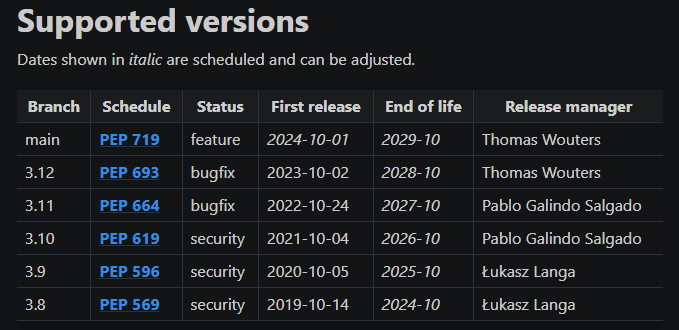
\includegraphics[width=0.5\linewidth]{Photos/Versoes-do-Python-4.png}
    \caption{Quadro de versões do \textit{Python} \cite{hashtagtreinamentos_python_versions}}
    \label{fig:enter-label}
\end{figure}

O \textit{Python} utiliza um esquema de versionamento conhecido como versionamento semântico \cite{hashtagtreinamentos_python_versions}, que é atualmente um dos sistemas de versionamento mais reconhecidos \cite{wikipedia_versionamento}. Esse esquema é composto por três números separados por pontos: MAJOR.MINOR.PATCH. O número MAJOR indica grandes mudanças que não são compatíveis com versões anteriores que possuem um número MAJOR diferente. O número MINOR é usado para adicionar funcionalidades compatíveis com a versão MAJOR atual. Já o número \textit{PATCH} refere-se a mudanças menores, como correções de \textit{bugs} e ajustes \cite{wikipedia_versionamento}.

No \textit{Python}, todas as versões possuem um status, que pode ser um dos seguintes: \textit{feature}, \textit{bugfix} ou \textit{security}. Quando uma versão está no status \textit{security}, significa que ela aceita apenas atualizações de segurança. Se uma versão está no status \textit{bugfix}, ela permite atualizações para correção de \textit{bugs} e também para segurança. Por último, o status \textit{feature} indica que a versão está aceitando atualizações que incluem novas funcionalidades \cite{hashtagtreinamentos_python_versions}.


\subsection{Versão 2.0}
A primeira versão significativa do \textit{Python} foi a 2.0, amplamente adotada pela comunidade de desenvolvedores. Ela trouxe recursos inovadores para a linguagem, como \textit{list comprehensions}, \textit{generators} e \textit{decorators} \cite{awari_python_version}.

\subsection{Versão 3.0}
Lançada em 2008, a versão 3.0 representa uma atualização significativa em relação à versão 2.0. Ela resolveu vários problemas e limitações da versão anterior, além de implementar diversas melhorias. As mudanças incluíram a eliminação da distinção entre strings e bytes, suporte nativo a Unicode e melhor gerenciamento de memória \cite{awari_python_version}.

\subsection{Versão 3.5}
Lançada em 2015, a versão 3.5 introduziu melhorias importantes, como a adição do operador de matriz de índice e um suporte aprimorado para \textit{await/async} \cite{awari_python_version}.

\subsection{Versão 3.8}
Lançado em 2019, o Python 3.8 trouxe várias novas funcionalidades e melhorias. Uma das principais adições foi a atribuição de expressões de linguagem, que permite atribuir valores a variáveis com base em expressões condicionais. Além disso, o Python 3.8 introduziu a possibilidade de usar o caractere de sublinhado como separador numérico para melhorar a legibilidade de números grandes \cite{awari_python_version}.
\section{Aplicações}

Python possui uma vasta gama de possibilidades para suas aplicações em projetos de Inteligência Artificial (IA), desde análise profunda de textos até automóveis autônomos, isso se faz possível pela sua grande quantidade de bibliotecas e também por sua simplificada metodologia de aplicação.\cite{didatica2024}

\subsection{Análise profunda de textos}

A análise profunda de textos, realizada através da mineração de textos, é uma aplicação comum de IA que utiliza \textit{Python}. Bibliotecas como NLTK e TextBlob permitem aos desenvolvedores analisar o tom emocional por trás de palavras e frases em grandes conjuntos de dados, abrindo portas para \textit{insights} em áreas como mercado de ações, avaliações de produtos e tendências de opinião pública possibilitando assim a extração de sentimentos dos textos.\cite{didatica2024}

\subsection{Automovéis Autônomos}

Python também desempenha um papel fundamental no desenvolvimento de tecnologias para veículos autônomos. Através de bibliotecas como OpenCV para processamento de imagens e \textit{TensorFlow} para aprendizado de máquina, desenvolvedores conseguem criar sistemas complexos de reconhecimento de padrões e tomada de decisão, essenciais para a navegação autônoma.\cite{didatica2024}
\section{Conclusão}
Em conclusão, Python se consolidou como uma ferramenta essencial na área de Inteligência Artificial, impulsionando inovações em diversas subáreas, como aprendizado de máquina, processamento de linguagem natural e visão computacional. Sua simplicidade, extensibilidade e suporte por uma vasta gama de bibliotecas especializadas tornam Python a escolha preferida tanto para pesquisa quanto para aplicações comerciais em IA. A linguagem continuará a desempenhar um papel crucial no avanço das tecnologias de IA, facilitando o desenvolvimento de soluções mais inteligentes e eficientes.
%\include{chap3}


\bibliographystyle{apalike}
\bibliography{referencias}
%\begin{thebibliography}{99}
    %\bibitem{almeida} Almeida, H. P., {\it Introdução a Teoria dos Códigos}, Editora da UFPB, 1999.
    %\bibitem{silva} Silva, A. A., {\it Matemática Elementar}, notas de aula, 1997.
%\end{thebibliography}




\end{document}